\documentclass[10pt]{standalone}
\usepackage{commands}
\begin{document}
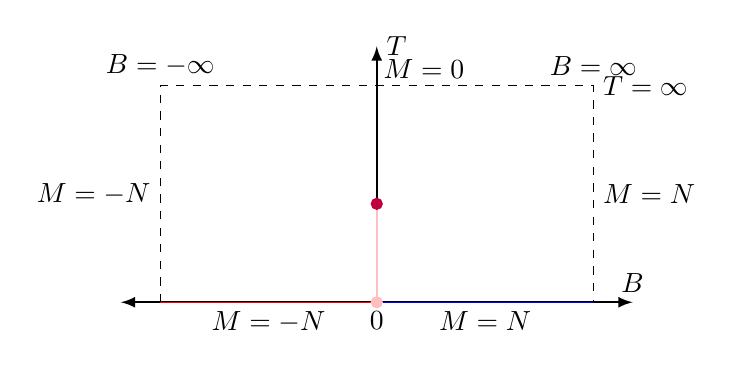
\begin{tikzpicture}
    \draw[thick, -latex] (0, 0) -- (0, 3.25);
    \draw[thick, latex-latex] (-3.25, 0) -- (3.25, 0);
    \draw[dashed] (-2.75, 0) -- (-2.75, 2.75) -- (2.75, 2.75) -- (2.75, 0);
    \node[right] at (0, 3.25) {$T$};
    \node[above] at (3.25, 0) {$B$};
    \node[above] at (-2.75, 2.75) {$B = -\infty$};
    \node[above] at (2.75, 2.75) {$B = \infty$};
    \node[right] at (2.75, 2.75) {$T = \infty$};
    \node[below] at (0, 0) {0};
    \node[left] at (-2.75, 1.375) {$M = -N$};
    \node[right] at (2.75, 1.375) {$M = N$};
    \node[below] at (0.6, 3.2) {$M=0$};
    \draw[red] (-2.75, 0) -- (0, 0);
    \draw[blue] (0, 0) -- (2.75, 0);
    \filldraw[pink] (0, 0) circle (2pt);
    \node[below] at (-1.375, 0) {$M = -N$};
    \node[below] at (1.375, 0) {$M = N$};
    \draw[thick, pink] (0, 0) -- (0, 1.25);
    \filldraw[purple] (0, 1.25) circle (2pt);
\end{tikzpicture}
\end{document}